\documentclass{article}
\usepackage{amsmath}
\usepackage{graphicx} % Required for inserting images
\graphicspath{ {./images/}




\title{Lab 1}

\begin{document}

\maketitle

\section{Text 1}

This is text. This is text. This is text. This is text. This is text. This is text. This is text. This is text. This is text. This is text. This is text. This is text. This is text. This is text. This is text. This is text. This is text. This is text. This is text. This is text.  This is text. This is text. This is text. This is text.


\section{Math 1}

This is a function:
\begin{equation}
    f(x) = x^2 - i + \pi
\end{equation}

This is a system of equations:

    \begin{equation}\label{system_eq_option_delta}
        \begin{cases}
            (\Pi_{0}-\Delta_{0}X_{0})(1+r) + \Delta_{0}X_{1}(H) = V_{1}(H),\\
            (\Pi_{0}-\Delta_{0}X_{0})(1+r) + \Delta_{0}X_{1}(T) = V_{1}(T).
        \end{cases}
    \end{equation}

\section{Image 1}


An image of a brick wall taken in Tbilisi, Georgia

\begin{figure}
    \centering
    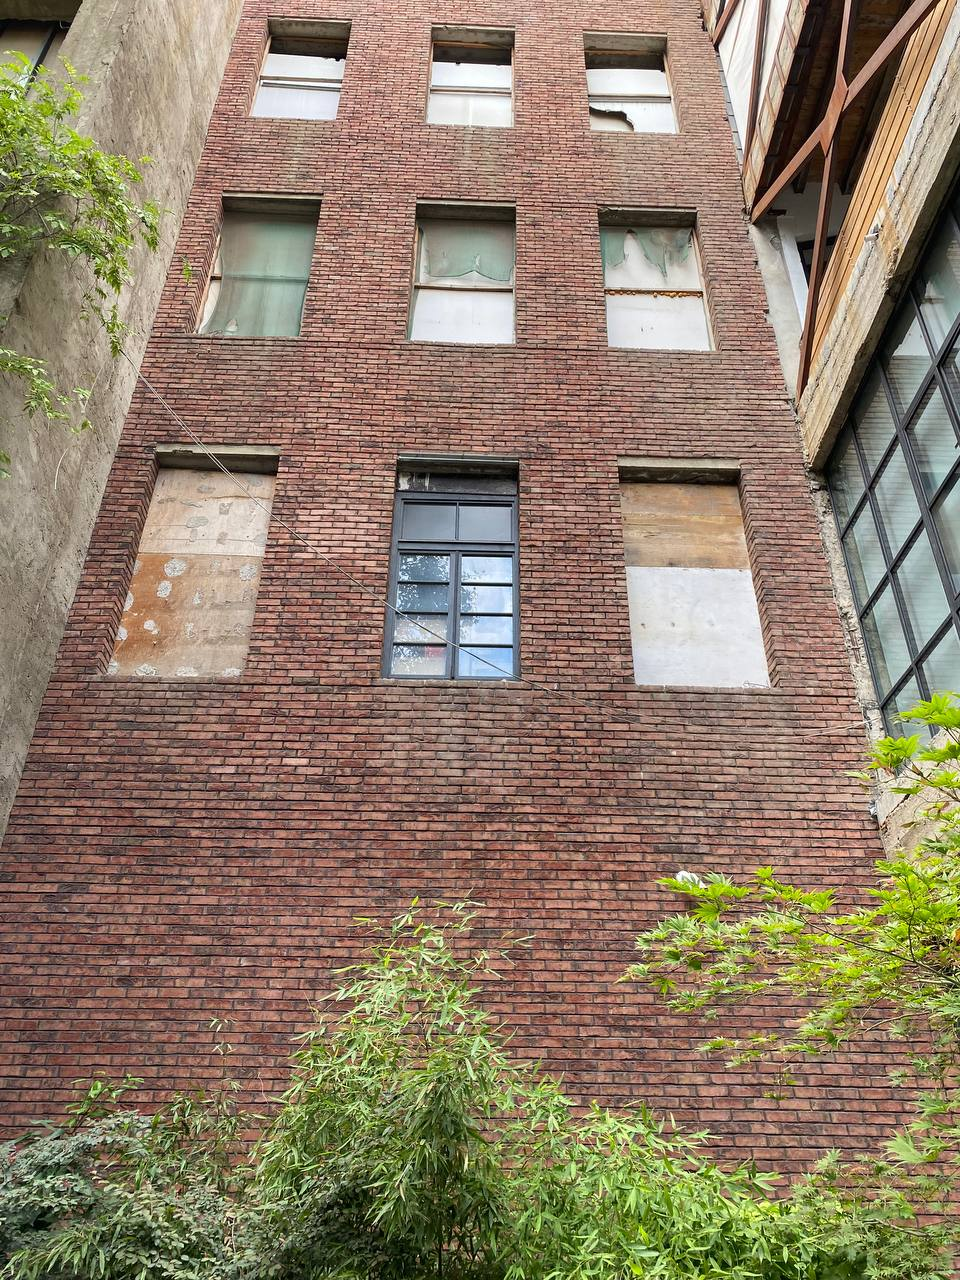
\includegraphics[width=0.25\textwidth]{brick_wall.jpg}
\end{figure}


\section{Text 2}

Another random text.

\large{Text.} \Large{Text.} \LARGE{Text.} \Large{Text.} \large{Text.}

\textbf{Text.} \textit{Text.} \textsc{Text.}

\section{Math 2}

\begin{equation}\nonumber
    V_{n}(\omega_1\omega_2...\omega_n)=\frac{V_{n+1}(\omega_1\omega_2...\omega_n H)\widetilde{p} + V_{n+1}(\omega_1\omega_2...\omega_n T)\widetilde{q}}{1+r},
\end{equation}
\begin{equation}\nonumber
    X_{n}(\omega_1\omega_2...\omega_n)=\frac{X_{n+1}(\omega_1\omega_2...\omega_n H)\widetilde{p} + X_{n+1}(\omega_1\omega_2...\omega_n T)\widetilde{q}}{1+r}.
\end{equation}


From my paperwork on the Dirichlet Problem for the Upper Half-Space:
\[
\begin{aligned}
|u(z)-f(a)|&=\left|\int_{\mathbf{R}^{n-1}}(f(t)-f(a)) P_{H}(z, t) d t\right| \\
\leq & \int_{|t-a| \leq \delta}|f(t)-f(a)| P_{H}(z, t) d t \\
&+2\|f\|_{\infty} \int_{|t-a|>\delta} P_{H}(z, t) d t
\end{aligned}
\]
for every $z \in H .$ If $\delta$ is small enough, then integral on $\{|t-a| \leq \delta\}$ is small too due to continuity $f$ in the point $a$ and due to $7.1 .$ The integral on $\{|t-a|>\delta\}$ converges to 0 when $z \to a$ due to the Proposition 7.2.



\end{document}
